\chapter{Radar and Meteorology}
\label{sec:meteorology}

For most of the 20th and early 21st century, weather radar has provided the highest resolution and most complete snapshot of meteorological phenomena. 
Some recent work has illuminated methods for developing even higher resolution weather data solutions by analyzing cellular communications data, but for most in the academic realm of geosciences, weather radar remains the most trusted and most available instrument for observing the atmosphere and meteorological phenomena.

Since this work focuses on identifying and classifying meteorological phenomena in weather radar scans, some discussion is warranted on what features can be observed in this data format, how humans analyze weather radar data, and solidifying the terminology used throughout this document.

\section{Precipitation Regimes}
\label{sec:meteorology_precip}

Essentially, we examine two major precipitation regimes: stratiform, and convection.
Examples drawn from the hand-labeled dataset of scans observed by the XMDL radar in the CASA DFW network are shown in Figure \ref{fig:meteorology_examples}.

\begin{figure}[h]
	\centering
	\begin{subfigure}[b]{0.45\textwidth}
		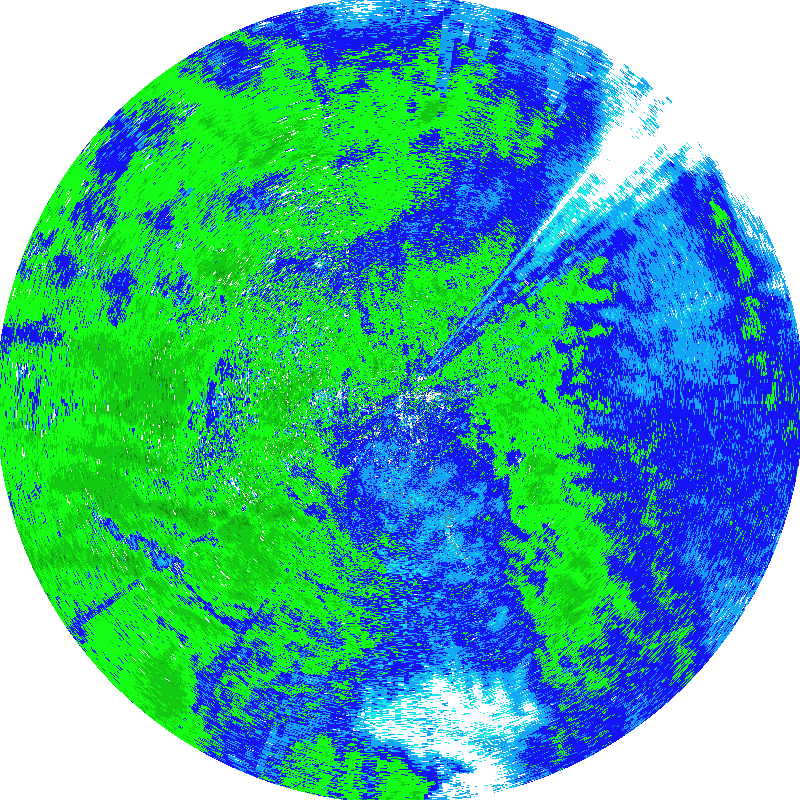
\includegraphics[width=\textwidth]{./thesis_code/plots/midlothian-tx-20170807-052557-ref-STRATIFORM.png}
		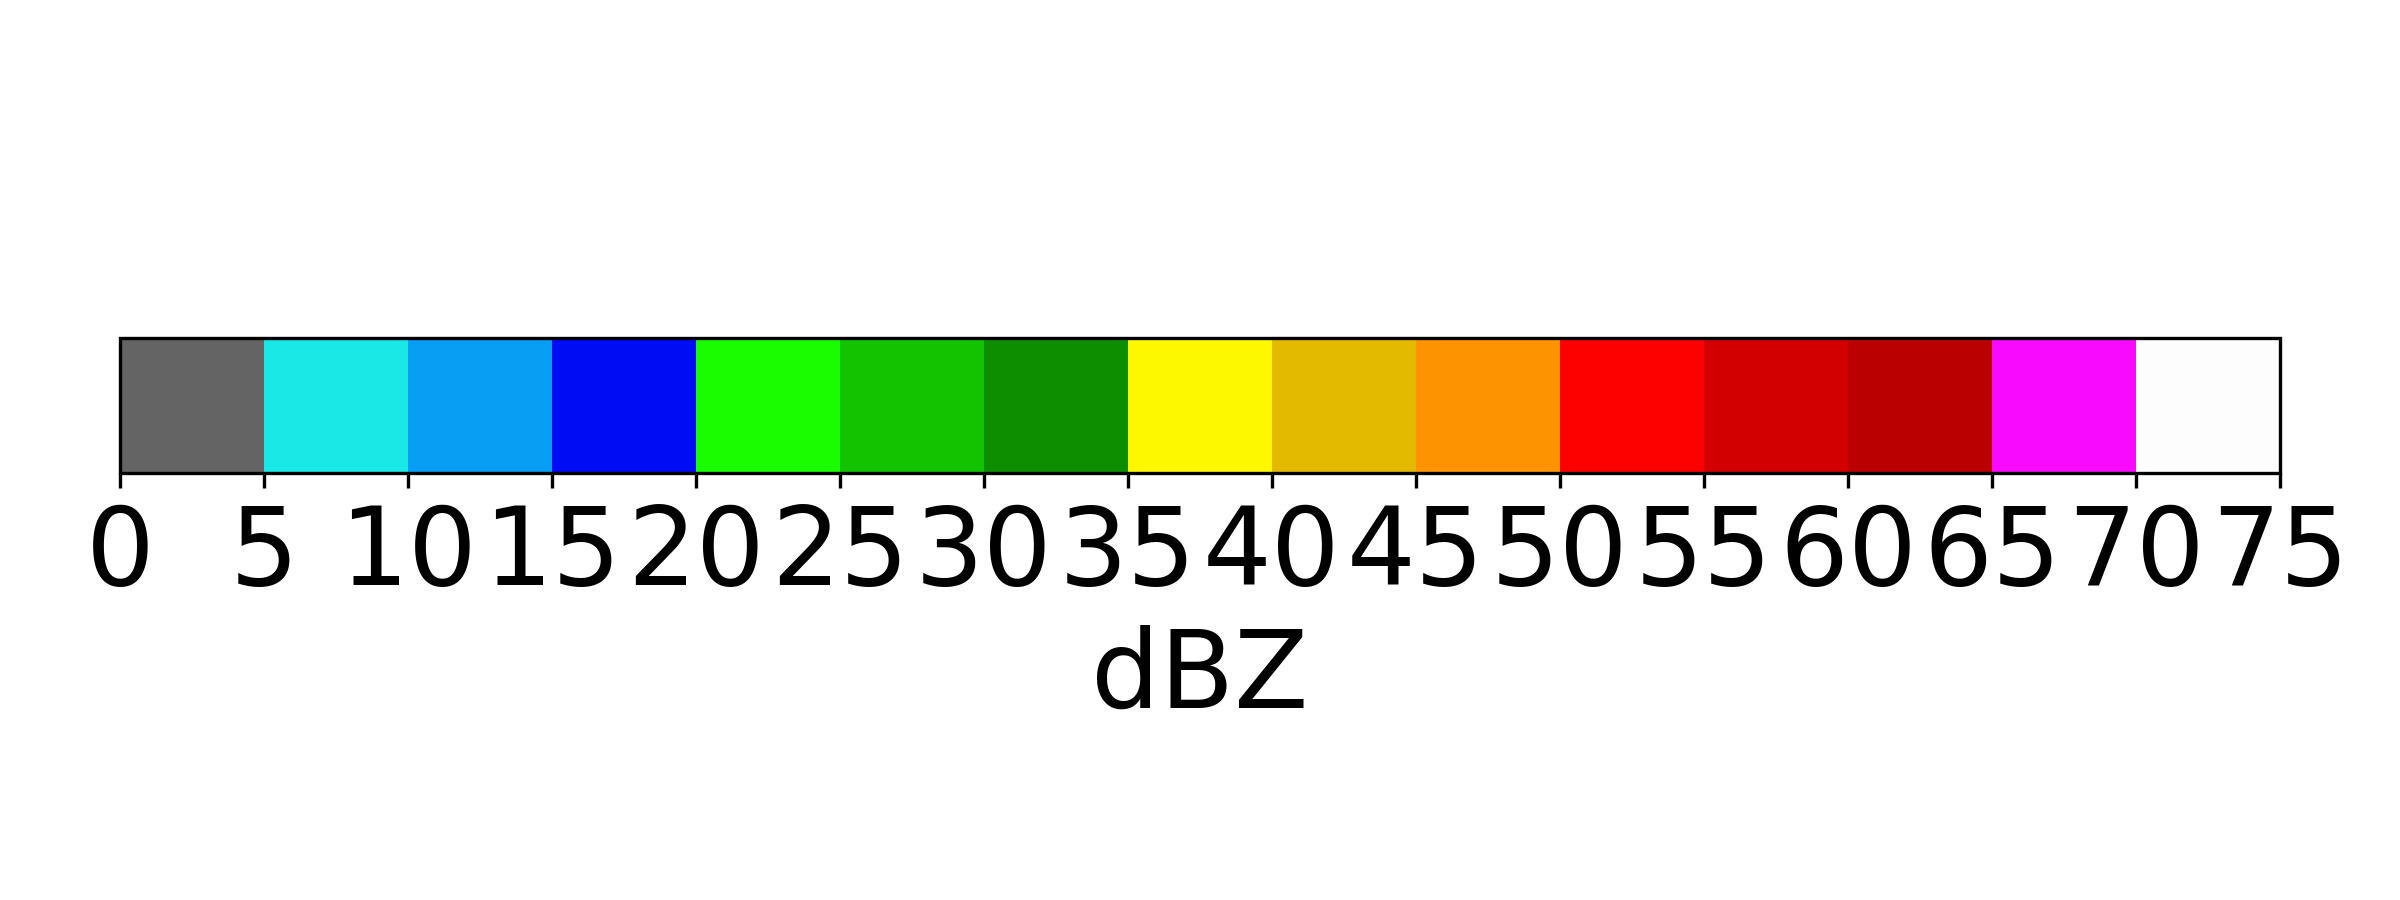
\includegraphics[width=\textwidth]{./thesis_code/plots/dfw_colormap.png}
		\caption{Stratiform - 2017-08-07 06:30:34 UTC}
		\label{fig:meteorology_stratiformexample}
	\end{subfigure}
	\begin{subfigure}[b]{0.45\textwidth}
		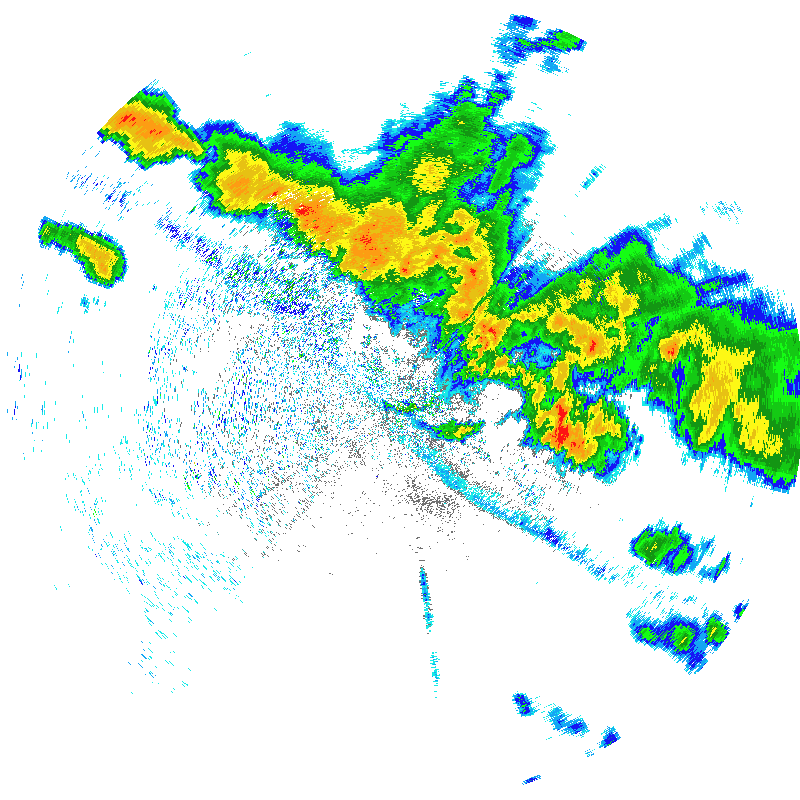
\includegraphics[width=\textwidth]{./thesis_code/plots/midlothian-tx-20170624-063034-ref-CONVECTION.png}
		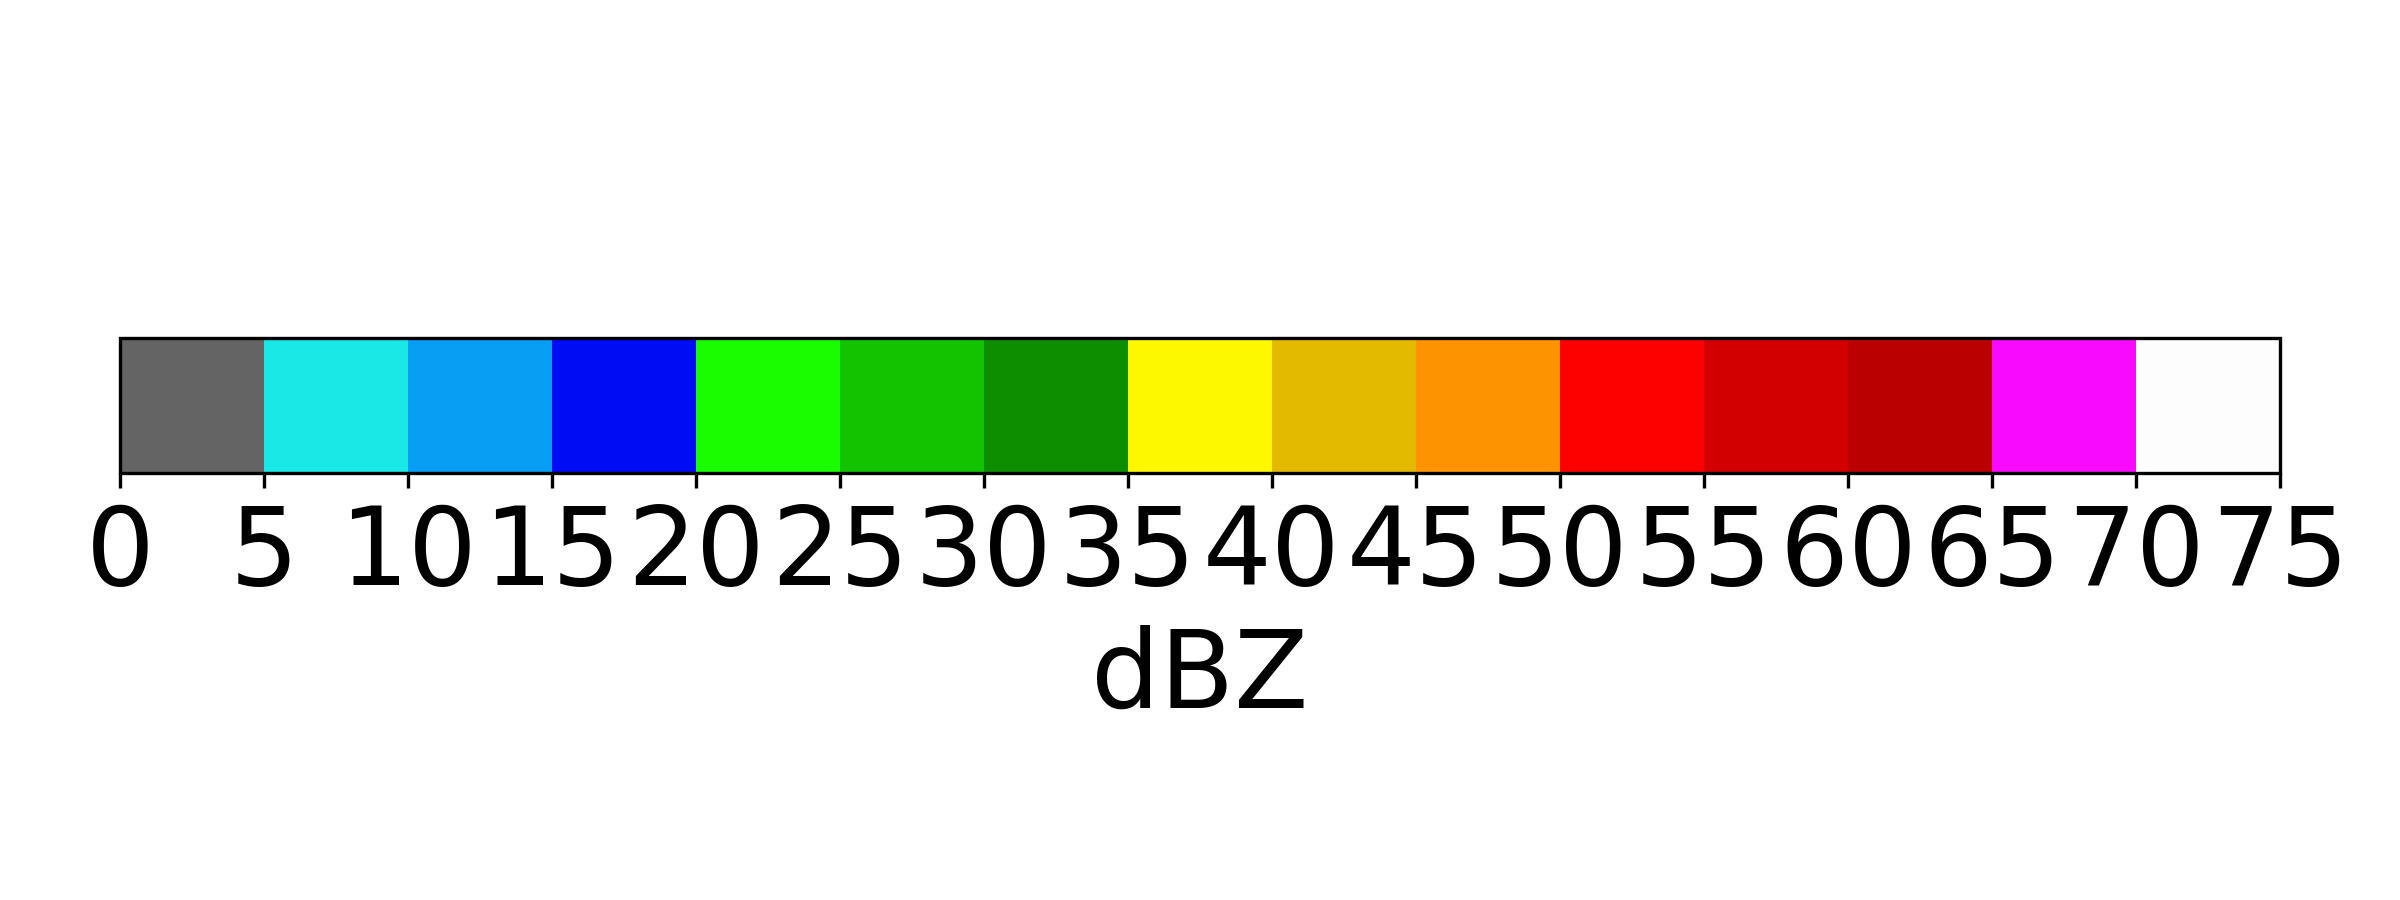
\includegraphics[width=\textwidth]{./thesis_code/plots/dfw_colormap.png}
		\caption{Convection - 2017-08-07 05:25:57 UTC}
		\label{fig:meteorology_convectionexample}
	\end{subfigure}
	\caption{Examples of radar reflectivity $Z_h$ from the two major precipitation regimes, observed by the XMDL radar in the CASA DFW network}
	\label{fig:meteorology_examples}
\end{figure}

Unfortunately, there is no hard and fast definition for what either of these particular regimes are.
It would be satisfying to be able to point out a few membership functions for radar parameters, as well as some specific atmospheric generating processes, as a way to conveniently put every precipitation radar scan into one of the two bins.
In fact, the former must be done to produce a training dataset, but it is worth noting here that this is something of a fiction.

\section{Radar Observations of Meteorological Echoes}
\label{sec:meteorology_echoes}

% combine the two sections above? I think so. Or just delete section{weather phenomena}

The highly cited ($>$ 650) "Stratiform Precipitation in Regions of Convection: A Meteorological Paradox?"\cite{houze1997stratiform} published in 1997 in the Bulletin of the American Meteorological Society attempts to provide a definition for stratiform precipitation, that we will use as a basis for the analysis in this work.
To wit: 
"Stratiform precipitation is fairly homogeneous in the horizontal, giving it a layered structure in vertical cross sections of radar reflectivity. In particular, it often exhibits a pronounced layer of high reflectivity called the "bright band," marking the layer in which the downward settling ice particles are melting."
Additionally, the authors contrast this with convection, which they aver can be detected on radar scans via pronounced cells of high reflectivity, corresponding to \textit{storm cells}, another term with loose definition.
The paper points out that storm cells typically feature spatially localized intense returns, that when viewed vertically in a range-height indicator (RHI) scan, appear to have a much taller core, and less pronounced bright band, than do the more spatially uniform stratiform precipitation scans.

It is with this knowledge that we turn our attention to plan-position indicator (PPI) scans, where elevation is fixed, and the radar scans in azimuth. 
In these scans, especially at lower elevation angles, there is far less of a chance to see a bright band, or melting layer.
However, stratiform regimes tend to produce more spatially uniform reflectivity returns over a large coverage area, whereas convection regimes produce cells of intense precipitation or hail, and correspondingly intense reflectivity returns, over smaller areas.
One final possibility is that convection can occur within a largely stratiform region, so there is overlap, from the perspective of the bulk image classification.

Other research efforts have attempted to use horizontal reflectivity data from PPI scans in classifying the two regimes. 
Along with pointing out the meteorological interest in discerning data of this type, \cite{biggerstaff2000improved} presents an algorithm that itself improved upon a prior work \cite{steiner1995climatological} via the Tropical Rainfall Measuring Mission (TRMM) to partition stratiform and convective regions within individual volumetric scans. 
This latter work points out the difficulty in using the melting layer identification as a method for performing stratiform vs convection classification: namely,

\begin{enumerate}
	\item Vertical resolution of weather radar scans (in PPI mode) are inadequate to resolve the melting layer except near the radar, limiting the sampling area
	\item The melting layer is not always well-developed even in stratiform regimes, especially in early-stage or late-stage stratiform, or in scans where both types of precipitation are present
\end{enumerate}

The authors describe a condition for the determination of stratiform precipitation in terms of a vertical updraft wind speed $w$:

\begin{equation}
|w| << |V_t|
\end{equation}

where $V_t$ is the snow particle terminal velocity, for particles above the melting layer.
In convection, this updraft speed is higher with respect to the fall speed, leading to particles growing in a different manner, and generating much larger rain drops or hail by the time they reach the ground.

By inference, and as stated above, in stratiform rain cases, precipitation is more spatially uniform than in convection, and this fact is utilized by \cite{steiner1995climatological} to perform classifications using the horizontal structure of the precipitation field. 
They convert the polar weather radar volume scan to a three-dimensional Cartesian grid, then look for peaks in the rain rate, which is directly proportional to reflectivity.
By defining and combining criteria regarding the intensity of reflectivity values, the number of peaks outside a convective center, and statistics from the surrounding area of the convective center, they make classifications regarding precipitation types in scans for specific regions.

This method utilizes information about the atmospheric processes and how they present in the highest resolution data available to perform classifications. 
However, its reliance on well-calibrated rain rate returns, available only via empirical determination and variable not only between locations but also in time limits the utility of this method in producing high fidelity classifications for other radars.
Furthermore, its statistics regarding reflectivity field values may not correspond to optimal discriminating functions for the two regimes, a drawback in any method that relies on heuristics, design choices, and other hyperparameters to determine a suitable function.

As we will discuss in Chapter \ref{sec:classifying}, one advantage in utilizing machine learning algorithms as tools for functional approximation is that many of the above design choices, parameters, and nonlinear mappings can be learned by models well-suited to the task.
This is not a new concept, of course, and early attempts using neural networks have been tried by other groups for performing these classifications. 
In one example \cite{anagnostou2004convective}, a shallow, three layer neural network consisting of two hidden layers of 8 neurons each was developed and trained on a set of features chosen by the authors.
The features included storm height, reflectivity values at specific elevations above ground level, height of maximum reflectivity level, vertical gradient of reflectivity, and horizontal reflectivity standard deviation.
This last feature ties in directly to the discussion above, whereby variable spatial returns may be less likely to be considered stratiform precipitation regimes.

As above, the classification was performed on WSR-88 reflectivity data, but this study utilized radars throughout the southeastern United States, as compared to only one platform in the previous regime.
Compared to the aforementioned methods, the false alarm rate in classifying stratiform was comparable, but was far superior to classifying convective precipitation than the others.
And false alarm rate (FAR) is perhaps the most important metric when considering data discovery, where the results of any algorithm are expected to represent the class that the algorithm labels them.
This study also demonstrated the value in utilizing neural networks as a functional approximation technique, and their strength in finding feature spaces where decisions can be more readily made.

The neural network in \cite{anagnostou2004convective} was impressive but only could learn a linear function, given its structure.
Additionally, the features in the network were drawn from a low-resolution 2 km x 2 km grid, which may have smoothed over local variability of interest.
Finally, the feature engineering provided valuable predictors, yet overlooked the raw two-dimensional textures inherent in radar reflectivity data, that form a large component of how humans perform precipitation regime classification.

Other methods have been shown to perform this classification and include instruments other than weather radar, such as disdrometers \cite{caracciolo2006analysis} and satellites \cite{feidas2012classifying}.
These systems are vaulable tools and can provide information to those with access to the data, but require either specialized instruments to implement, or correspond to smaleler-than-desireable coverage areas than weather radar, and as such will be ignored in this analysis.
